\chapter{Appendix}




% Please add the following required packages to your document preamble:
% \usepackage{multirow}
% \usepackage{graphicx}
\begin{table}[ht]
\centering
\caption{Results from statistical online evaluation Of variants}
\label{tab:online_stats}
\resizebox{\textwidth}{!}{%
\begin{tabular}{|l|lllllll|l|}
\hline
\multirow{2}{*}{\textbf{Variant}} & \multicolumn{7}{c|}{\textbf{Score}}                                                                                                                                                                                                      & \multirow{2}{*}{\textbf{Avg Time (s)}} \\ \cline{2-8}
                                  & \multicolumn{1}{l|}{\textbf{mean}} & \multicolumn{1}{l|}{\textbf{std}} & \multicolumn{1}{l|}{\textbf{min}} & \multicolumn{1}{l|}{\textbf{25\%}} & \multicolumn{1}{l|}{\textbf{50\%}} & \multicolumn{1}{l|}{\textbf{75\%}} & \textbf{max} &                                        \\ \hline
1                                 & \multicolumn{1}{l|}{18.76}         & \multicolumn{1}{l|}{6.97}         & \multicolumn{1}{l|}{8.0}          & \multicolumn{1}{l|}{14.25}         & \multicolumn{1}{l|}{17.5}          & \multicolumn{1}{l|}{21.0}          & 48.0         & 146.3                                  \\ \hline
2                                 & \multicolumn{1}{l|}{11.05}         & \multicolumn{1}{l|}{2.57}         & \multicolumn{1}{l|}{6.0}          & \multicolumn{1}{l|}{10.0}          & \multicolumn{1}{l|}{11.0}          & \multicolumn{1}{l|}{13.0}          & 15.0         & 154.75                                 \\ \hline
3                                 & \multicolumn{1}{l|}{12.54}         & \multicolumn{1}{l|}{1.9}          & \multicolumn{1}{l|}{10.0}         & \multicolumn{1}{l|}{11.0}          & \multicolumn{1}{l|}{13.0}          & \multicolumn{1}{l|}{15.0}          & 15.0         & 249.12                                 \\ \hline
4                                 & \multicolumn{1}{l|}{11.53}         & \multicolumn{1}{l|}{1.9}          & \multicolumn{1}{l|}{7.0}          & \multicolumn{1}{l|}{10.0}          & \multicolumn{1}{l|}{11.0}          & \multicolumn{1}{l|}{13.0}          & 15.0         & 71.42                                  \\ \hline
5                                 & \multicolumn{1}{l|}{26.82}         & \multicolumn{1}{l|}{8.48}         & \multicolumn{1}{l|}{12.0}         & \multicolumn{1}{l|}{20.0}          & \multicolumn{1}{l|}{27.0}          & \multicolumn{1}{l|}{33.0}          & 53.0         & 127.77                                 \\ \hline
6                                 & \multicolumn{1}{l|}{22.03}         & \multicolumn{1}{l|}{9.1}          & \multicolumn{1}{l|}{11.0}         & \multicolumn{1}{l|}{16.0}          & \multicolumn{1}{l|}{19.0}          & \multicolumn{1}{l|}{29.0}          & 51.0         & 79.91                                  \\ \hline
\end{tabular}%
}
\end{table}

\begin{table}[htpb]
\centering
\caption{Category and wording of survey questions}
\label{tab:survey_questions}
\resizebox{\textwidth}{!}{%
\begin{tabular}{|c|c|c|}
\hline
\textbf{Question category} &
  \textbf{Wording} &
  \textbf{Response Type} \\ \hline
\multirow{2}{*}{Travel Knowledge} &
  How often do you travel for vacation? &
  \multirow{2}{*}{5 points Likert Scale} \\ \cline{2-2}
 &
  How good are you at planning vacations? &
   \\ \hline
Scenario Match &
  What are your preferred travel experiences? &
  \begin{tabular}[c]{@{}c@{}}Multi Choice from\\ Beach, Watersports,\\ Entertainment, Shopping\\ Culinary, Hiking,\\ Nature \& Wildlife,\\ Cities \& Architecture\end{tabular} \\ \hline
Trust &
  \begin{tabular}[c]{@{}c@{}}Do you tend to trust a person/thing, even though \\ you have little knowledge of it\end{tabular} &
  \multirow{5}{*}{5 points Likert scale} \\ \cline{1-2}
Accuracy &
  The recommended regions matched the input preferences &
   \\ \cline{1-2}
Satisfaction &
  \begin{tabular}[c]{@{}c@{}}This recommender system gave me good suggestions \\ for this scenario\end{tabular} &
   \\ \cline{1-2}
Diversity &
  The regions recommended are diverse &
   \\ \cline{1-2}
Cohesiveness &
  The recommended regions fit well together &
   \\ \hline
\end{tabular}%
}
\end{table}


\begin{table}[htpb]
\centering
\caption{Dunn-Bonferroni-Tests for pairwise comparison between the travel knowledge of respondents.}
\label{tab:dunntest_knowledge_all}
\resizebox{\textwidth}{!}{%
\begin{tabular}{|l|l|l|l|l|l|}
\hline
\multicolumn{1}{|c|}{} & \textbf{Test Statistic} & \textbf{Std. Error} & \textbf{Std. Test Statistic} & \textbf{p} & \textbf{Adj. p} \\ \hline
Advanced - Average & 270.87 & 32.56 & 8.32 & \textless{}.001 & \textless{}.001 \\ \hline
Advanced - Basic   & 373.27 & 70.16 & 5.32 & \textless{}.001 & \textless{}.001 \\ \hline
Average - Basic    & 102.41 & 71.72 & 1.43 & .153            & .46             \\ \hline
\end{tabular}%
}
\end{table}

\begin{figure}
\begin{tabular}{cc}
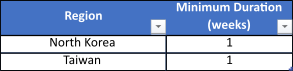
\includegraphics[width=.45\textwidth]{Alg1_input1} &  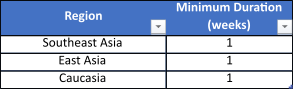
\includegraphics[width=.45\textwidth]{Alg4_input1} \\
(a) Variant 1 (baseline) & (b) Variant 4 \\[6pt]
 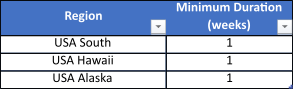
\includegraphics[width=.45\textwidth]{Alg5_input1} &   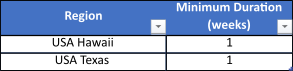
\includegraphics[width=.45\textwidth]{Alg6_input1} \\
(c) Variant 5 & (d) Variant 6 \\[6pt]
\end{tabular}
\caption{Recommendations generated for input scenario 1 per variant}\label{fig:input1_suggestions}
\end{figure}
\begin{figure}
\begin{tabular}{cc}
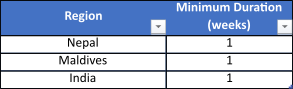
\includegraphics[width=.45\textwidth]{Alg1_input2} &  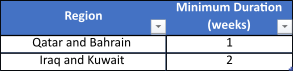
\includegraphics[width=.45\textwidth]{Alg4_input2} \\
(a) Variant 1 (baseline) & (b) Variant 4 \\[6pt]
 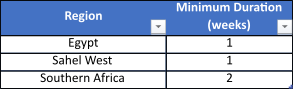
\includegraphics[width=.45\textwidth]{Alg5_input2} &   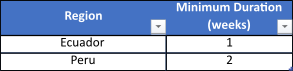
\includegraphics[width=.45\textwidth]{Alg6_input2} \\
(c) Variant 5 & (d) Variant 6 \\[6pt]
\end{tabular}
\caption{Recommendations generated for input scenario 2 per variant}\label{fig:input2_suggestions}
\end{figure}
\begin{figure}
\begin{tabular}{cc}
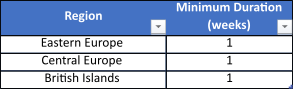
\includegraphics[width=.45\textwidth]{Alg1_input3} &  
\includegraphics[width=.45\textwidth]{Alg4_input3} \\
(a) Variant 1 (baseline) & (b) Variant 4 \\[6pt]
 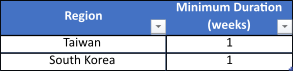
\includegraphics[width=.45\textwidth]{Alg5_input3} &   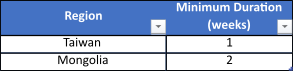
\includegraphics[width=.45\textwidth]{Alg6_input3} \\
(c) Variant 5 & (d) Variant 6 \\[6pt]
\end{tabular}
\caption{Recommendations generated for input scenario 3 per variant}\label{fig:input3_suggestions}
\end{figure}

\begin{figure}[htpb]
    \centering
    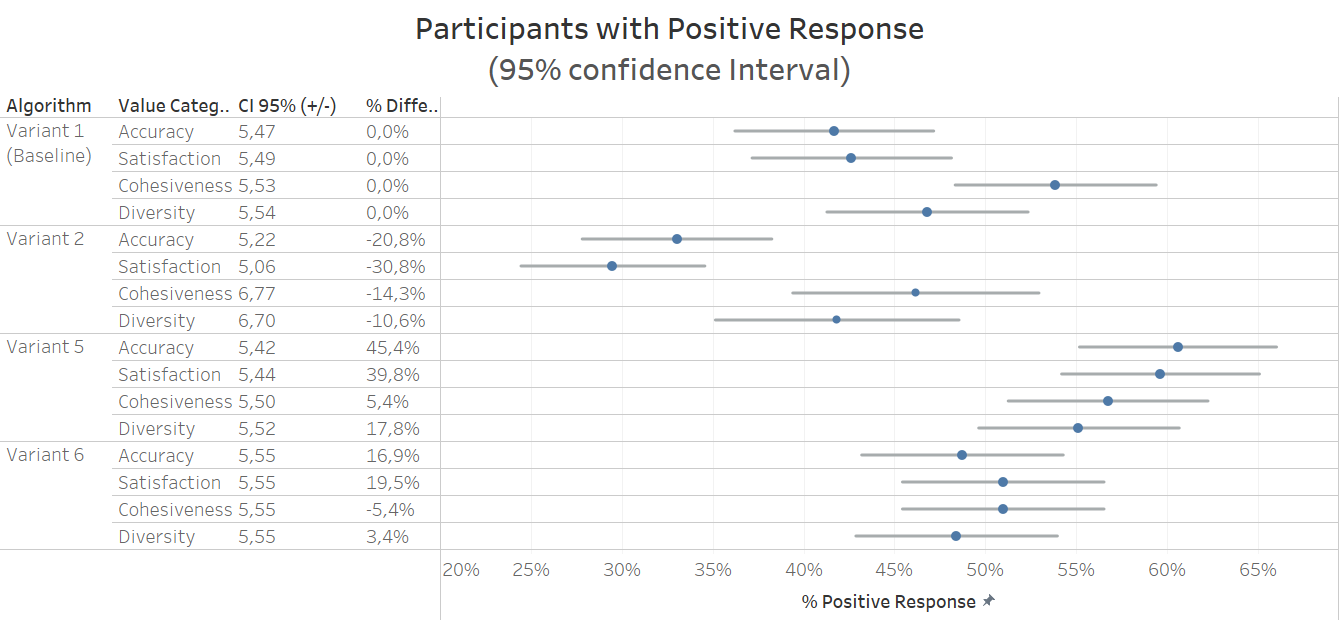
\includegraphics[width=\textwidth]{Survey_Statistical_Inference}
    \caption[Margin of error of results using 95\% Confidence Interval with 302 records per variant]
    {Margin of error in the results of the survey using a 95\% confidence interval on the positive responses; The percentage improvement of each record on the different categories compared to baseline is shown. The percentage improvement is calculated as the percentage difference for each category relative to the baseline. From the results obtained, we can ascertain with 95\% confidence that each variant will always generate the same results, with an approximately [-6, 6] margin of error.}
    \label{fig:survey_stat_inference}
\end{figure}



